% \begin{figure}[htb]	
% \center%6.3
% 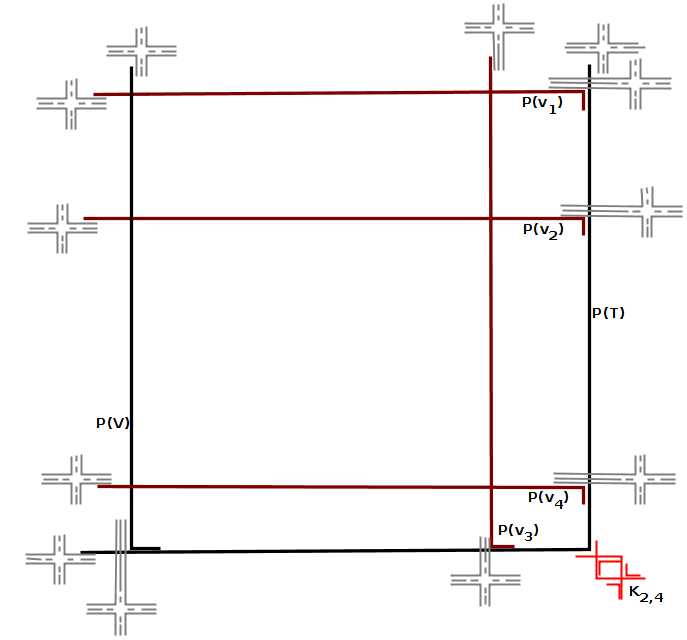
\includegraphics[width=10cm]{./img/gf3.png}
% %clausulaGadgetGFCompletaSBPO
% \caption{Single bend representation of the base and variables gadgets associated with the assignment $x_1=False, x_2=False, x_3=True, x_4=False$ }
% \label{fig:gadgetBasePlusVariables}
% \end{figure}
\begin{figure}[h]
  \centering
%segundo bloco de figuras
  \begin{tabular}{p{8cm} p{8cm}}
   \centering 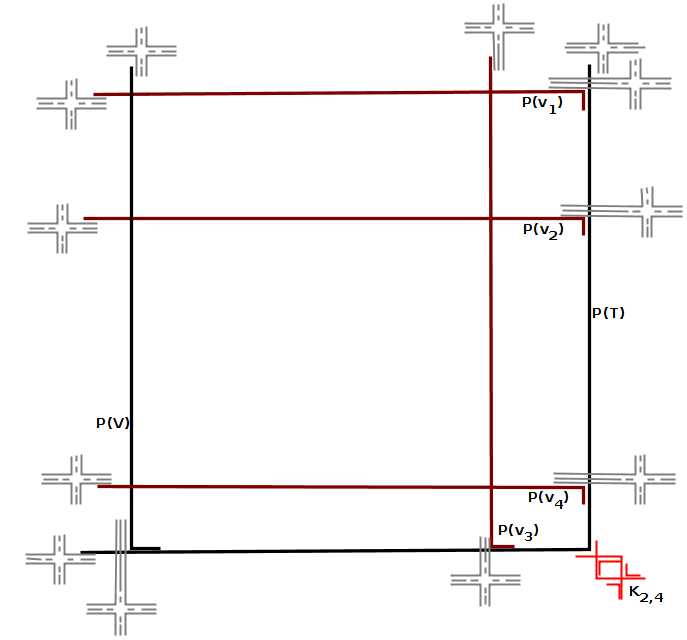
\includegraphics[width=8cm, left]{./img/gf3.png} & 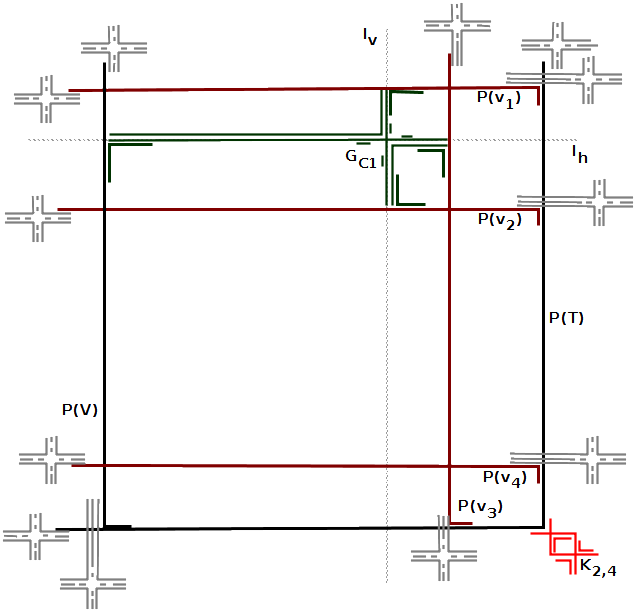
\includegraphics[width=8cm, left]{./img/formulaCompletaGFonePiePlusLines.png} \\  
  [\abovecaptionskip]
    \footnotesize \centering (a) Representation with omitted clause gadgets & \footnotesize(b) Representation with  $G_{C_1}$  associated with the clause $(x_1+x_2+x_3)$ in highlighted \\
%    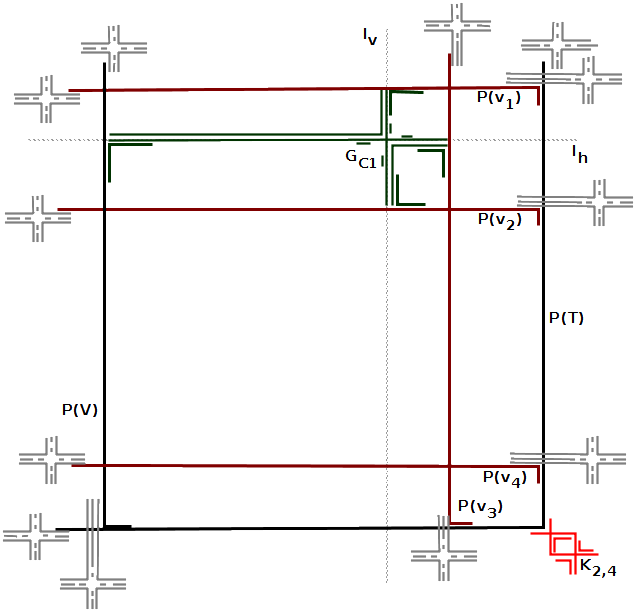
\includegraphics[width=10cm]{./img/formulaCompletaGFonePiePlusLines.png}
%   \\
%     \footnotesize(b) Representation with  $G_{C_1}$  associated with the clause $(x_1+x_2+x_3)$ in highlighted \label{fig:gadgetOnePie}
% \\
  \end{tabular}

 \caption{Single bend representation of the base and variables gadgets associated with the assignment $x_1=False, x_2=False, x_3=True, x_4=False$} \label{fig:gadgetOnePie} \label{fig:gadgetBasePlusVariables}
\end{figure}